\section{Auswertung}
\label{sec:auswertung}

\subsection{Längenbestimmung über Schallgeschwindigkeit in Acryl}
\label{subsec:längenbest}

Zunächst wurde die Dicke der Acrylplatte mithilfe einer Schieblehre zu
\begin{equation*}
    D_\text{m} = (10,0 \pm 0,05) \,\unit{\milli\meter}
\end{equation*}
bestimmt.

Um dann die Schallgeschwindigkeit zu ermitteln, wurden die Differenzen zwischen den einzelnen Peaks gemessen.
Wie in \autoref{fig:export1} zu erkennen, wurde das Messfenster so eingestellt, dass vier Impulse zu sehen waren.

\begin{figure}
    \centering
    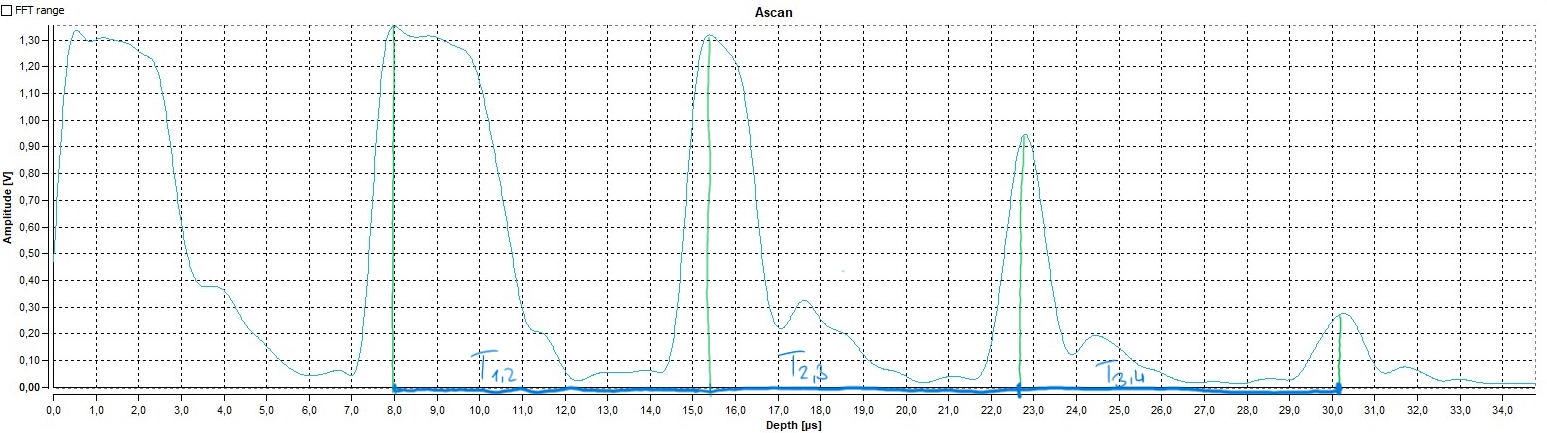
\includegraphics[width=\textwidth]{figures/MessungAcrylplatte(1).jpg}
    \caption{Screenshot der Impulsmessung aus \textit{FlowView}.}
    \label{fig:export1}
\end{figure}

Die Differenzen $T_{i,i+1}$ zwischen dem $i$-ten und $i + 1$-Peak kann dabei zur Schallgeschwindigkeitsberechnung genutzt werden, zur genaueren Bestimmung
der Differenzen wurde dabei die intgrierten Cursor auf je ein Peak-Paar gesetzt und die Differenz der x-Position abgelesen.
Dabei betrugen die Differenzen
\begin{align*}
    T_{1,2} &= 7,43 \,\unit{\micro\second} \,,\\
    T_{2,3} &= 7,41 \,\unit{\micro\second} \,,\\
    T_{3,4} &= 7,30 \,\unit{\micro\second} \,.\\
\end{align*} \\

Um während der Versuchsdurchführung Zeit zu sparen, wurde, um die Schallgeschwindigkeit zu berechnen, die Differenz $T_{1,2}$ als 'Mittelwert' gewählt,
mit der sich die Schallgeschwindigkeit aus \eqref{eq:schallges} zu
\begin{equation*}
    c = 2691,79 \,\unit{\frac{\meter}{\second}}
\end{equation*}
bestimmt. \\

Nach Eintragung der Schallgeschwindigkeit in \textit{FlowView} lässt sich die x-Achse auf eine Längenskala umstellen.
Wird erneut die Differenz zwischen zwei Peaks ermittelt, ergibt sich eine Länge von
\begin{equation*}
    D_\text{exp} = 10,52 \unit{\milli\meter} \,,
\end{equation*}
also eine Abweichung von
\begin{equation*}
    \frac{D_\text{exp}-D_\text{m}}{D_\text{m}} = 0,052 = 5,20 \,\% \,.
\end{equation*}


\subsection{Schallgeschwindigkeitsbestimmung in Acryl}

Um einen besseren Vergleich der Messwerte zu ermöglichen, sollen hier die Messwerte aus Impuls-Echo-Verfahren und Durchschallungsverfahren zusammengeführt werden.
Die aufgenommenen Messdaten, also die Zylinderdicken mit den dazugehörigen Laufzeiten, sind für das Impuls-Echo-Verfahren in \autoref{tab:1a}, für das Durchschallungsverfahren in \autoref{tab:1b} dargestellt.

\begin{table}[H]
    \begin{subtable}{0.5\textwidth}
        \centering
        \caption{Laufzeitbestimmung über Impuls-Echo-Verfahren.}
        \label{tab:1a}  
        \begin{tabular}{c c}
        \toprule 
        {Zylinderhöhe $h \mathbin{/} \unit{\milli\meter}$} & {Laufzeit $\Delta t \mathbin{/} \unit{\micro\second}$} \\
        \midrule 
         28,1      &       23,37       \\ 
         37,5      &       29,37       \\  
         65,6      &       23,11       \\
         77,5      &       59,17       \\ 
         99,1      &       75,85       \\ 
        114,6      &       59,05       \\
        117,8      &       88,33       \\  
        \bottomrule
        \end{tabular}   
    \end{subtable}
    \begin{subtable}{0.5\textwidth}
        \centering
        \caption{Laufzeitbestimmung über Durchschallungsverfahren.}
        \label{tab:1b} 
        \begin{tabular}{c c}
        \toprule 
        {Zylinderhöhe $h \mathbin{/} \unit{\milli\meter}$} & {Laufzeit $\Delta t \mathbin{/} \unit{\micro\second}$} \\
        \midrule 
         28,1       &       23,02       \\   
         37,5       &       28,90       \\
         65,6       &       23,11       \\   
         77,5       &       59,24       \\
         -          &       -           \\      
        114,6       &       23,02       \\ 
         -          &       -           \\
        \bottomrule
        \end{tabular}  
    \end{subtable}
 \caption{Zylinderdicken und Laufzeiten unter Impuls-Echo- sowie Durchschallungsverfahren.} 
\end{table}

Zu beachten sind dabei die fehlenden Messwerte beim Durchschallungsverfahren, die aufgrund fehlender Kompetenz auf Seiten der Messenden nicht aufgenommen werden konnten. \\

Wird eine lineare Regression der Form
\begin{equation*}
    y = c x + b
\end{equation*}
durchgeführt, wobei die Steigung $c$ die Schallgeschwindigkeit und der y-Achsenabschnitt $b$ die Anpassungsschicht darstellt, ergeben sich die in \autoref{fig:graph1a} und \autoref{fig:graph1b} dargestellten Plots.
    
\begin{figure}[H]
        \centering
        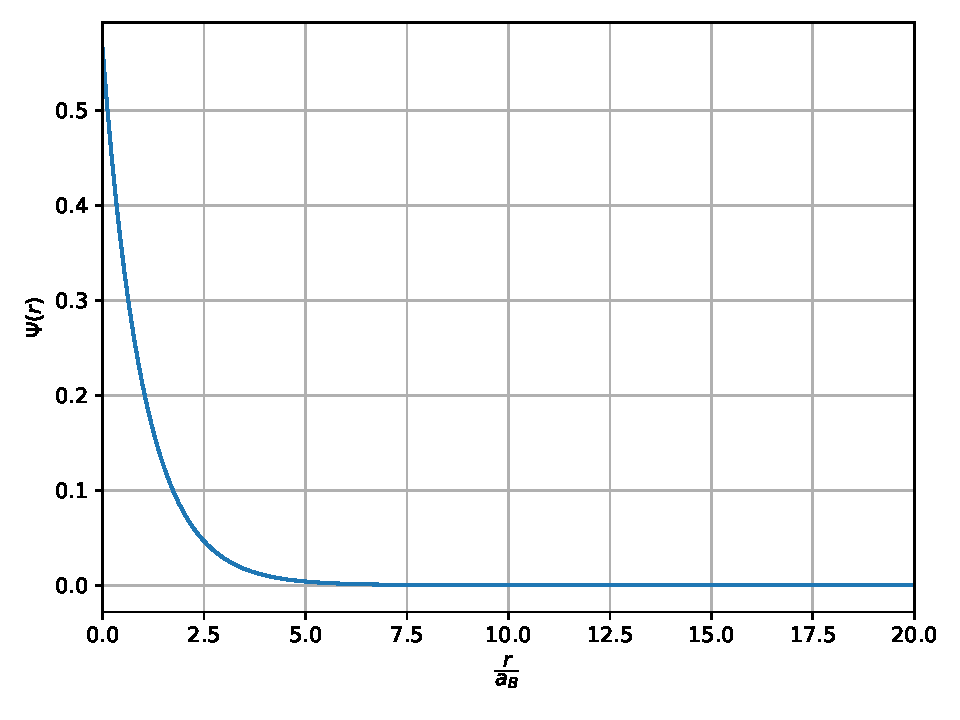
\includegraphics[width=\textwidth]{build/Graph_a.pdf} 
        \caption{Plot der Messdaten und Ausgleichsgeraden für das Impuls-Echo-Verfahren.}
        \label{fig:graph1a}
\end{figure}

Für das Impuls-Echo-Verfahren ergeben sich die Koeffizienten dabei zu
\begin{equation*}
    c = \left( 2361.67 \pm 598.61 \right) \,\unit{\frac{\meter}{\second}}
\end{equation*}
und
\begin{equation*}
    b = \left( 0.033 \pm 0.034 \right) \,\unit{\meter} \,.
\end{equation*}

\begin{figure}[H]
    \centering
    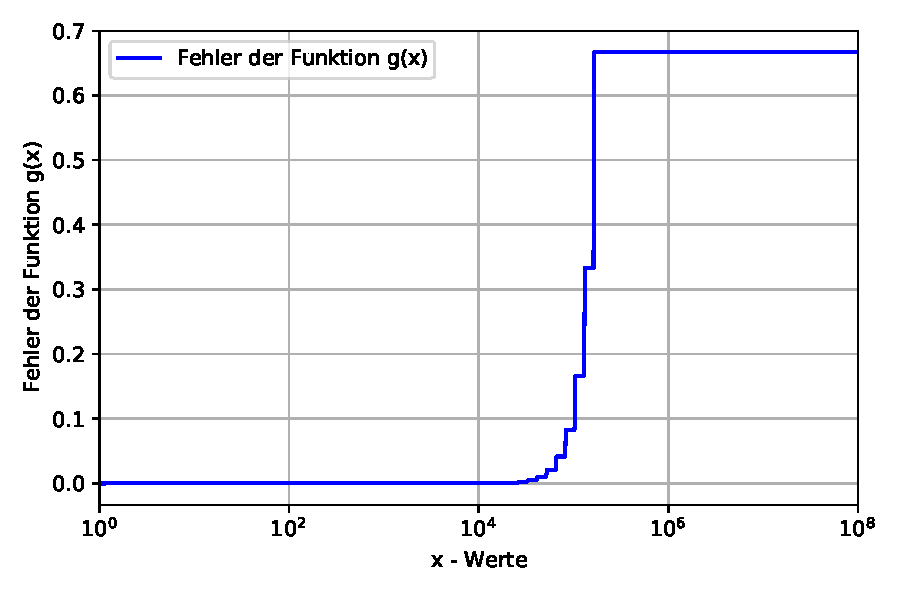
\includegraphics[width=\textwidth]{build/Graph_b.pdf} 
    \caption{Plot der Messdaten und Ausgleichsgeraden für das Durchschallungsverfahren.}
    \label{fig:graph1b}
\end{figure}

Hier ergeben sich für das Durchschallungsverfahren
\begin{equation*}
    c = \left( 308.387 \pm 1249.599 \right) \,\unit{\frac{\meter}{\second}}
\end{equation*}
und
\begin{equation*}
    b = \left( 0.0549 \pm 0.043 \right)\,\unit{\meter} \,.
\end{equation*} \\


\subsection{Bestimmung der Dämpfung mit Impuls-Echo-Verfahren}

Hier wird nun nicht länger die Zeitdifferenz zwischen zwei Einzelimpulsen, sondern die Amplitudendifferenz benötigt.
Analog zu \autoref{subsec:längenbest} werden die Cursor im Programm auf die beiden Impulspeaks gesetzt, anhand der Anzeige kann einfach die Amplitudendifferenz
als Differenz auf der y-Achse abgelesen werden.
Dabei wurde die Verstärkung vollständig abgeschaltet.
Die Amplitude des ersten und zweiten Impulses, die Amplitudendifferenz sowie die Höhe des jeweils verwendeten Zylinders bzw. 
der verwendeten Zylinderkombination sind in \autoref{tab:2}
dargestellt.

\begin{table}
    \centering
    \caption{Amplitudendifferenzen über das Impuls-Echo-Verfahren.}
    \label{tab:2} 
    \begin{tabular}{c c c c}
    \toprule 
    {Zylinderhöhe $h \mathbin{/} \unit{\milli\meter}$} & {$A_1 \mathbin{/} \unit{\volt}$} & {$A_2 \mathbin{/} \unit{\volt}$} & {$\Delta A \mathbin{/} \unit{\volt}$}\\
    \midrule 
     28,1       &       1,343       &        1,243      &       0,100       \\       
     37,5       &       1,347       &        1,278      &       0,069       \\       
     65,6       &       1,341       &        1,157      &       0.184       \\       
     77,5       &       2,136       &        0,445      &       1,681       \\       
    105,6       &       1,327       &        0,077      &       1,250       \\
    115,0       &       1,324       &        0,086      &       1,238       \\               
    \bottomrule
    \end{tabular}  
\end{table}

Die Regression erfolgt dabei über den exponentiellen Zusammenhang
\begin{equation*}
    I(l) = I_0 \text{e}^{-2 \cdot \alpha l} \,,
\end{equation*}
der in \autoref{fig:graph2} dargestellte Plot trägt die Zylinderlänge gegen den Logarithmus der Amplitude auf. \\
Dabei sind
\begin{align*}
    \alpha  &= (5.087 \pm 0.974) \,\frac{1}{\unit{\meter}} \,.
\end{align*}

\begin{figure}[H]
    \centering
    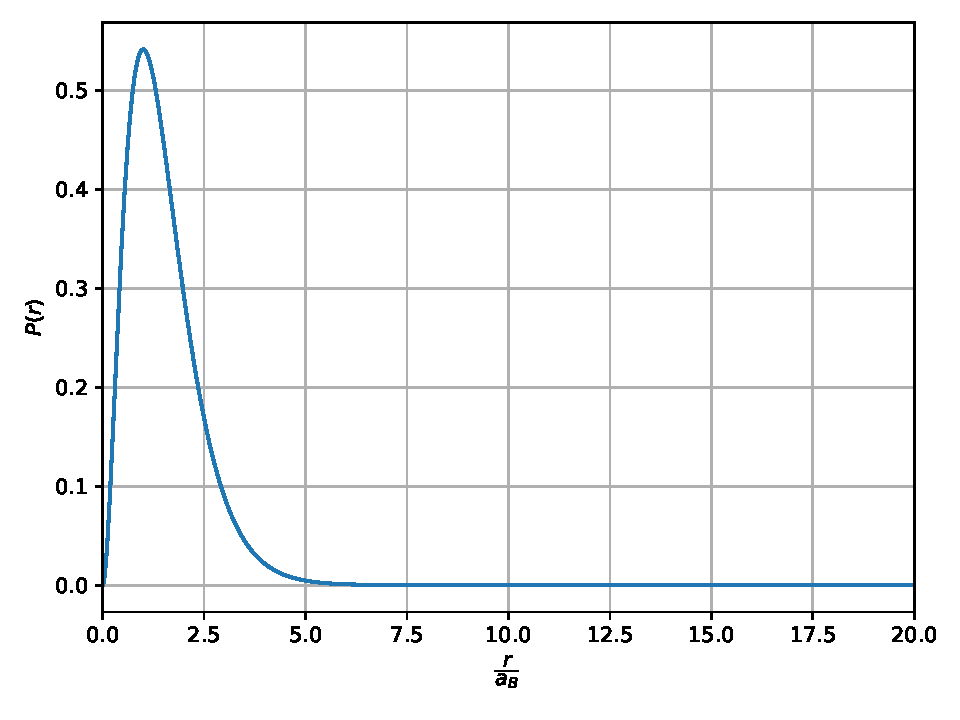
\includegraphics{build/Graph_c.pdf}
    \caption{Zylinderlänge l gegen Logarithmus der Amplitude $U$.}
    \label{fig:graph2}
\end{figure}

\newpage

\subsection{Vermessung des Augenmodells}


Zur Vermessung des Augenmodells wurden die Laufzeiten bis zur Iris sowie bis zur Retina aufgenommen. Das Augenmodel ist dreimal so groß wie ein echtes Auge. 
Nach \eqref{eq:schallges} ergeben sich mit $c_\text{L} = 2500 \,\unit{\frac{\meter}{\second}}$, der Schallgeschwindigkeit in der Linse, und
$c_\text{GK} = 1410 \,\unit{\frac{\meter}{\second}}$, der Schallgeschwindigkeit in der Glaskörperflüssigkeit, die in \autoref{tab:3} dargestellten Werte.


\begin{table}
    \centering
    \caption{Laufzeiten und Abmessungen im Auge.}
    \label{tab:3} 
    \begin{tabular}{| c | c |}
    \hline 
    {$\Delta t_\text{Iris} \mathbin{/} \unit{\micro\second}$}    &       9,06   \\
    {$l_\text{Iris} \mathbin{/} \unit{\meter}$}                  &       0,0113 \\
    {$\Delta t_\text{Retina} \mathbin{/} \unit{\micro\second}$}  &      16,13   \\
    {$l_\text{Retina} \mathbin{/} \unit{\meter}$}                &       0,0276 \\
    \hline
    \end{tabular}  
\end{table}